\documentclass{beamer}
\usepackage[T1,plmath]{polski}
\usepackage[utf8]{inputenc}
\usepackage{graphicx}
\usepackage{amsfonts}
\usepackage{amsmath}
\usepackage{amssymb}
\usepackage{amsthm}

\usepackage{float}
\usepackage[font=small,labelfont=bf]{caption}

% Theme choice:
\usetheme{Warsaw}

% Title page details: 
\title{Pamięć podręczna (ang. \emph{cache}) i jej wykorzystanie przy optymalizacji programów równoległych.} 
\author{Rafał Lenart}
\date{\today}


\begin{document}

% Title page frame
\begin{frame}
    \titlepage 
\end{frame}


% Outline frame
\begin{frame}{Outline}
    \tableofcontents
\end{frame}


% Lists frame
\section{Budowa pamięci operacyjnej w komputerze}
\begin{frame}{Jaka pamięć?}
	Jaka powinna być pamięć operacyjna?
	\begin{enumerate}
	\pause
	\item Szybka
	\pause
	\item Stabilna
	\pause
	\item Pojemna
	\pause
	\item Tania
	\end{enumerate}
\end{frame}


\begin{frame}{Rodzaje pamięci RAM}
% W idealnym świecie chcemy żeby pamięć operacyjna była tania, szybka, stabilna i jeszcze pojemna.
% Rzeczywistość: -_-
Pamięć ram dzieli się na dwa rodzaje.
\begin{enumerate}
    \item \textbf{DRAM} - Dynamic RAM
    \item \textbf{SRAM} - Static RAM
\end{enumerate}

\end{frame}

\begin{frame}{1 bit pamięci DRAM}
  \begin{minipage}{0.5\textwidth}
    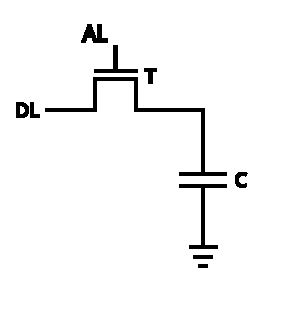
\includegraphics[scale=1]{assets/DRAM_bit.pdf}
  \end{minipage}%
  \begin{minipage}{0.5\textwidth}
  	\begin{itemize}
  		\item $AL$ - linia adresująca
  		\item $DL$ - linia danych
  		\item $T$ - tranzystor
  		\item $C$ - kondensator
  	\end{itemize}
  	\pause
  	\centering
  	\vspace{20px}
  	\textbf{Co tu jest problemem?}
    
  \end{minipage}
\end{frame}

\begin{frame}{Cechy DRAM}
  \begin{minipage}{0.5\textwidth}
    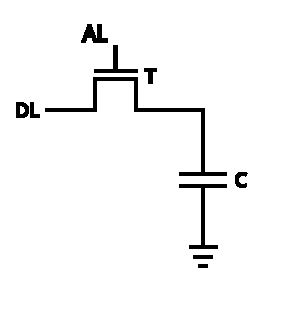
\includegraphics[scale=1]{assets/DRAM_bit.pdf}
  \end{minipage}%
  \begin{minipage}{0.5\textwidth}
	Cechy DRAM:
	\begin{itemize}
		\pause
		\item Tylko jeden tranzystor na bit.
		\pause
		\item Potrzebuje odświeżania ("wyciekający" ładunek).
		\pause
		\item Wartość wyjściowa jest analogowa.
		\pause
		\item Jest używany w	zewnętrznych układach.	
	\end{itemize}
  \end{minipage}
\end{frame}

\begin{frame}{1 bit pamięci SRAM}
	  \begin{minipage}{0.6\textwidth}
    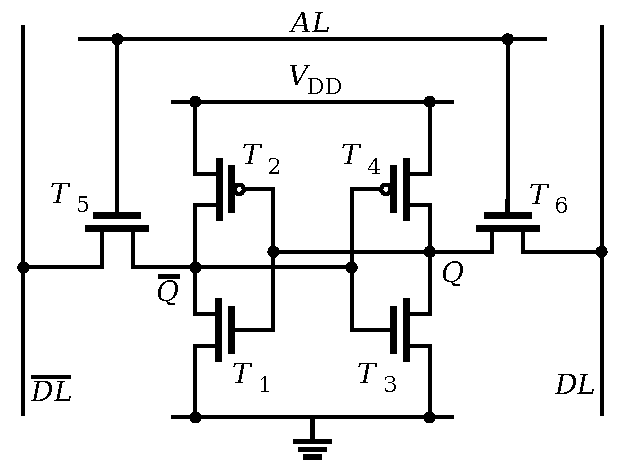
\includegraphics[scale=0.6]{assets/SRAM_bit.pdf}
  \end{minipage}%
  \begin{minipage}{0.4\textwidth}
  	\begin{itemize}
  		\item $AL$ - linia adresująca
  		\item $DL$ - linia danych
  		\item $T_{1-6}$ - tranzystory
  		\item $V_{DD}$ - Napięcie zasilające
  		\item $Q$ - Ładunek z przerzutnika
  	\end{itemize}
  \end{minipage}
\end{frame}

\begin{frame}{Cechy SRAM}
	  \begin{minipage}{0.6\textwidth}
    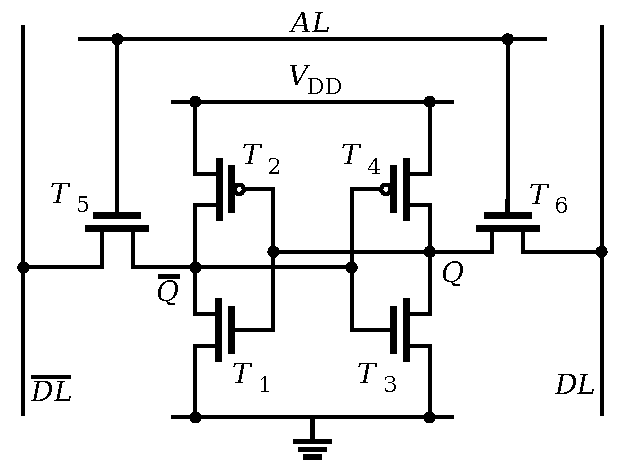
\includegraphics[scale=0.6]{assets/SRAM_bit.pdf}
  \end{minipage}%
  \begin{minipage}{0.4\textwidth}
  Cechy SRAM:
  	\begin{itemize}
		\pause
		\item Aż 6 tranzystorów na każdy bit.
		\pause
		\item Wymaga stałego zasilania $V_{DD}.$
		\pause
		\item Wartości na wyjściach są cyfrowe.
		\pause
		\item Dostęp do wartości w czasie mniejszym niż 1ns.
  	\end{itemize}
  \end{minipage}
\end{frame}

\section{Pamięć podręczna}
\begin{frame}{Do czego nam pamięć podręczna?}
Wiemy już następujące rzeczy:
\begin{itemize}
	\item statyczny RAM jest drogi, mało pojemny ale bardzo szybki
	\item dynamiczny RAM jest tani, bardzo pojemny ale stosunkowo wolny.
\end{itemize}
\pause
\begin{block}{Pytanie:}
Jak zatem uzyskać dużą pojemności pamięci operacyjnej, zachowując przy tym wysoką prędkość?
\end{block}
\pause
\begin{exampleblock}{Odpowiedź:}
Poprzez wykorzystanie \textbf{pamięci podręcznej} (cache).
\end{exampleblock}

\end{frame}
\begin{frame}{Czym jest pamięć podręczna?}
\begin{block}{Cache}
\textbf{Cache} to segment pamięci służącej do przechowywania kopii danych z pamięci o większej pojemności, do których dostęp będzie potrzebny w najlbiższej przyszłości.
\end{block}

Współczesne procesory często mają kilka poziomów pamięci podręcznej.
\end{frame}

\begin{frame}{Adresowanie}
Adresy w pamięci cache często są 64 bitowymi wartościami które są podzielone na 3 części jak na rysunku poniżej.
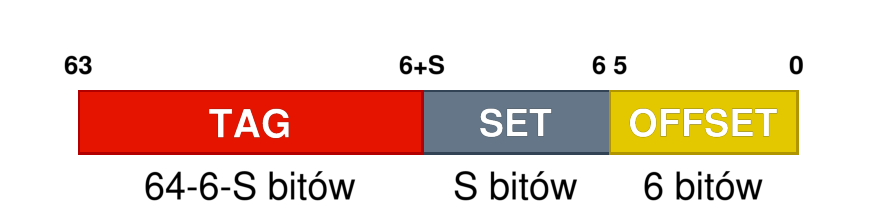
\includegraphics[scale=0.75]{assets/cache_address.pdf}
OFFSET to adresowanie poszczególnych bitów w wybranej poprzez SET oraz TAG linii pamięci podręcznej (ang. \emph{cache line}). 6 bitów przeznaczonych jest dla nią dla tego że zwykle linia jest 64 bitowa.

\end{frame}

\begin{frame}{Adresowanie}
Liczba S bitów przeznaczona na zbiór linii jest wyznaczana w zależności od tego ilo-"drożny" jest cache (ang. \emph{n-way cache}).
\begin{exampleblock}{Przykład}
Weźmy pod uwagę przypadek gdzie linia ma 64 bity, pamięć jest 8-drożna i jej pojemność to 64KB. Chcemy znaleźć liczbę S bitów w sekcji SET adresu. Każdy zbiór zawiera w sobie 8 linii (dlatego, że pamięć 8-drożna) więc jeden zbiór zawiera $16*8=128$ bajtów. pojemność całego cache-u to $64KB$ więc istnieje $64KB/128B = 512$ zbiorów. Dla podanego przykładu $S = 9$ ponieważ $2^9 = 512$.
\end{exampleblock}
\end{frame}

\begin{frame}{Adresowanie}
    \centering
    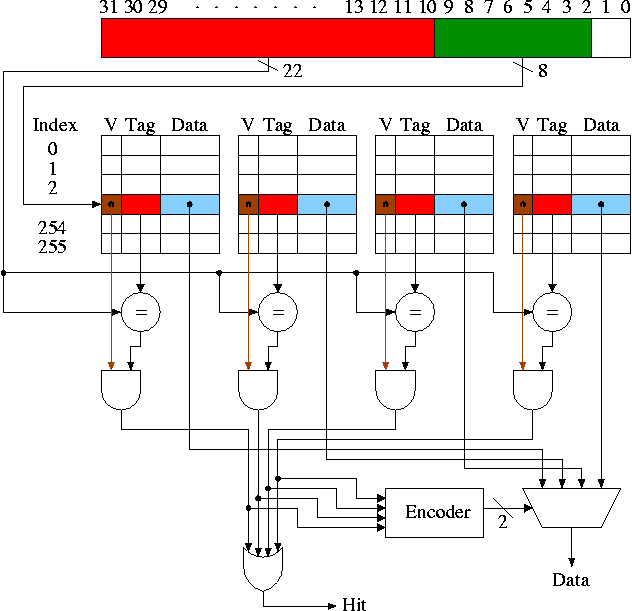
\includegraphics[scale=0.3]{assets/cache_4way.png}
\end{frame}

\begin{frame}{Po co kilka poziomów?}
Obecnie procesory mają zwykle 3 lub nawet 4 poziomy pamięci podręcznej. Dzieje się tak dlatego, że wraz ze zwiększaniem wielkości bloku pamięci, zwiększa się także opóźnienie związane z adresowaniem, a także rozmiar multiplekserów na kostce procesora. Poziomowanie rozwiązuje też do pewnego stopnia kwestię jednoczesnego dostępu do pamięci gdyż najniższe poziomy pamięci podręcznej (L0 - L1 - L2) są osobne dla każdego rdzenia, podczas gdy cache L3 jest współdzielony.
\end{frame}

\begin{frame}{Hierarchia poziomów cache}
\centering
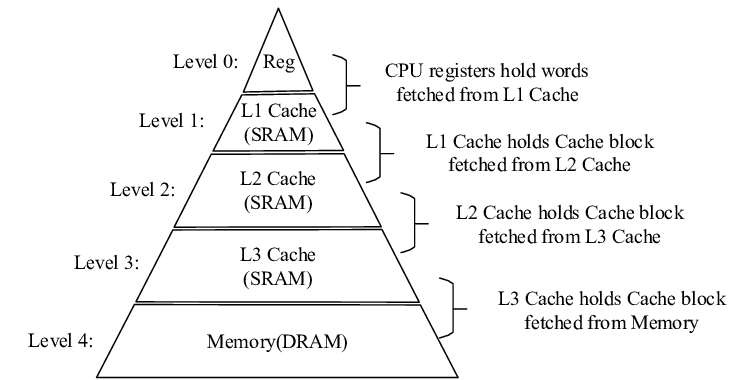
\includegraphics[scale=1]{assets/cache_hierarchy.png}
\end{frame}

\begin{frame}{Poziomy cd.}
Przykładowo procesory z serii Ryzen 7000 mają kolejno
\begin{itemize}
    \item L1 cache – 64 KB na rdzeń
    \item L2 cache – 1 MB na rdzeń
    \item L3 cache – 32 to 128 MB współdzielone
\end{itemize}

\end{frame}

\begin{frame}{Poziomy cd.}
    Podczas próby dostępu do pamięci procesor w pierwszej kolejności szuka jej w najniższym poziomie pamięci podręcznej (zwykle nazwanej L0 lub L1). Jeśli nie znaleziono tych danych które były potrzebne, następuje \textbf{cache miss} i dane szukane są dalej w wyższych poziomach pamięci.
\end{frame}

\section{Równoległość}
\begin{frame}{Równoległość a pamięć podręczna}
Jakie problemy należy rozwiązać przy podzieleniu pamięci podręcznej na różne poziomy?
\pause
\begin{itemize}
    \item Co się dzieje przy zapisie?
    \pause
    \item Jak uzyskać spójny obraz pamięci podręcznej dla każdego rdzenia w procesorze?
\end{itemize}
\end{frame}

\begin{frame}{MESI}

Z pomocą przychodzi protokół MESI. Jego założeniem jest przypisywanie do każdej linii pamięci podręcznej jednego z czterech stanów:
\pause
\begin{itemize}
    \item M (modified) - linia pamięci jest dostępna tylko w jednym z poziomów cache i jest różna od zawartości pamięci głównej.
    \pause
    \item E (exclusive) – linia pamięci jest dostępna tylko w jednym z poziomów cache, oraz w pamięci operacyjnej
    \pause
    \item S (shared) – linia pamięci jest dostępna na wszystkich poziomach cache oraz w pamięci operacyjnej
    \pause
    \item I (invalid) – linia pamięci jest nieaktualna i może zostać zastąpiona inną.
\end{itemize}
\end{frame}

\begin{frame}{Diagram przejść w MESI}
\centering
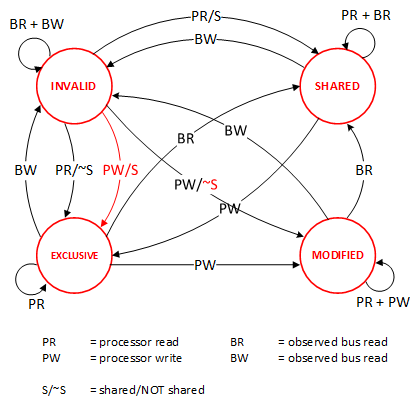
\includegraphics[scale=0.6]{assets/MESI.png}
\end{frame}

\begin{frame}{Co robić?}
\begin{itemize}
    \item Dobre wykorzystywanie pamięci podręcznej
    \begin{itemize}
    \pause
        \item utrzymywać małe bloki danych.
    \pause
        \item próbować skanować liniowo.
    \pause
        \item unikać skakania po wskaźnikach.
    \end{itemize}
    \pause
    \item Prefetching
    \begin{itemize}
    \pause
        \item Prefetching to pobieranie danych w dużych kawałkach przewidując ich wykorzystanie w bliskim czasie.
        \pause
        \item umożliwiać procesorowi automatyczny prefetching
        \pause
        \item dokonywać tego samodzielnie (trudniejsze zagadnienie)
    \end{itemize}
\end{itemize}
\end{frame}

\begin{frame}{Źródła}
\begin{itemize}
    \item \url{https://www.youtube.com/watch?v=4_smHyqgDTU}
    \item \url{https://www.akkadia.org/drepper/cpumemory.pdf}
    \item \url{https://cs.nyu.edu/~gottlieb/courses/2000s/2001-02-fall/arch/lectures/lecture-22.html}
    \item
    \url{https://pl.wikipedia.org/wiki/MESI}
\end{itemize}
\end{frame}


\end{document}